% Here you describe the empirical procedure followed to apply your algorithms to
% obtain answers to the goals/hypothesis of the study. You elaborate on the
% performance measures used and provide the benchmark problems used. Provide all
% control parameter values with a motivation for why you have used these, and
% state the number of independent runs. If statistical tests are used, these are
% discussed here. After reading this section (in addition to the background) the
% reader should be able to duplicate your experiments to obtain similar results
% to those obtained by you.
\section{Empirical Procedure}
\label{sec:empirics}

This section presents the five datasets, examines their temporal patterns and
stationarity, and explains the construction of the synthetic AR(2) series.

\subsection{Datasets and Stationarity Analysis}
\label{sec:datasets}

To comprehensively evaluate and compare the Elman, Jordan, and Multi-recurrent
neural network architectures, five time series benchmark problems are selected.
These datasets embody distinct dynamic regimes, including deterministic trends,
multi-frequency seasonality, short-term physical persistence, decadal cycles,
and stationary linear stochastic dependence. In this section, we analyze the
four empirical time series benchmarks, examine their visual patterns, and
formally evaluate their stationarity properties using rolling statistics, the
Autocorrelation Function (ACF), the Augmented Dickey-Fuller (ADF) unit-root
test~\cite{DickeyFuller1979}, and the Kwiatkowski-Phillips-Schmidt-Shin (KPSS)
stationarity test~\cite{KPSS1992}. A synthetic second-order autoregressive
process, AR(2), is selected as the fifth dataset.

\begin{figure*}[t]
  \centering
  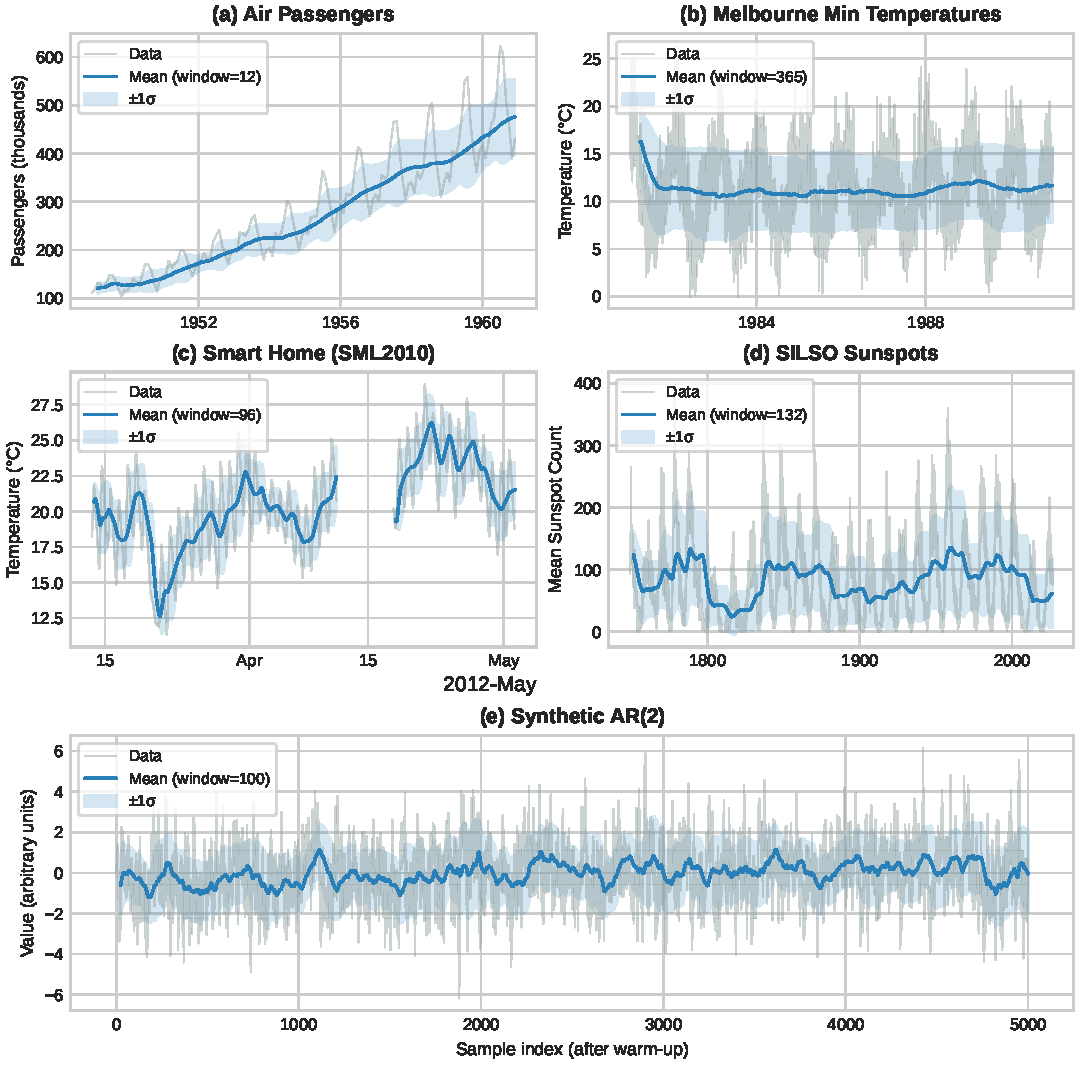
\includegraphics[width=0.95\textwidth]{figures/target_features_all.pdf}
  \caption{Target feature trajectories for all five benchmark datasets: (a) International Airline Passengers with 12-month rolling mean and $\pm 1\sigma$ band; (b) Melbourne Daily Minimum Temperatures with 365-day rolling statistics; (c) Smart Home (SML2010) dining-room temperature with 24-hour (96-step) rolling statistics across both recording segments; (d) SILSO Monthly Sunspot Numbers with 132-month (approximately 11-year) rolling statistics; (e) synthetic AR(2) with 100-sample rolling statistics, indexed after discarding warm-up samples. Shaded bands show rolling mean $\pm 1$ rolling standard deviation, not confidence intervals. The AR(2) smoothing window does not represent a seasonal period.}
  \label{fig:target_features}
\end{figure*}

\begin{table*}[t]
\centering
\footnotesize
\caption{Empirical Stationarity and Descriptive Diagnostics for the Four Time Series Datasets}
\label{tab:stationarity}
\begin{tabular*}{\textwidth}{@{\extracolsep{\fill}}lccccccp{4.2cm}}
\toprule
\textbf{Dataset} & \textbf{Obs ($N$)} & \textbf{Mean $\pm$ Std} & \textbf{ACF(1)} & \textbf{ACF(Cycle)} & \textbf{ADF ($p$)} & \textbf{KPSS ($p$)} & \textbf{Primary Evidence} \\
\midrule
Air Passengers & 144 & 280.3 $\pm$ 119.5 & 0.948 & 0.760 (12) & 0.82 (0.992) & 1.65 (0.010) & \textbf{Non-stationary} (trend and growing variance); ADF $p>0.99$, KPSS $p<0.01$. \\
Melbourne Min Temps & 3,652 & 11.2 $\pm$ 4.1 & 0.774 & 0.480 (365) & -4.44 (0.000) & 0.06 (0.100) & \textbf{Non-stationary} (annual cycle $s=365$, $\text{ACF}(365)=0.48$); time-varying mean. \\
Smart Home (Dining) & 2,764 & 19.2 $\pm$ 2.9 & 0.999 & 0.742 (96) & -5.34 (0.000) & 1.17 (0.010) & \textbf{Non-stationary} (diurnal cycle $s=96$, $\text{ACF}(96)=0.74$); level shifts, KPSS $p<0.01$. \\
SILSO Sunspots & 3,332 & 82.2 $\pm$ 67.6 & 0.918 & 0.553 (132) & -10.71 (0.000) & 0.11 (0.100) & \textbf{Cyclical / Mixed} (solar cycle $s\approx 132$, $\text{ACF}(132)=0.55$); decadal amplitude modulation. \\
\bottomrule
\end{tabular*}
\end{table*}


A weakly stationary time series possesses a time-invariant mean
$\mathbb{E}[y_t] = \mu$, a constant variance
$\mathrm{Var}(y_t) = \sigma^2 < \infty$, and an autocovariance
$\mathrm{Cov}(y_t, y_{t-k}) = \gamma_k$ that depends strictly on the temporal
lag $k$ rather than the absolute calendar time $t$. Table~\ref{tab:stationarity}
reports descriptive properties and statistical test outcomes, while
Fig.~\ref{fig:target_features} depicts the observed trajectories alongside
rolling central tendencies and volatility bands.

\subsubsection{International Airline Passengers}
The monthly airline passengers dataset~\cite{BoxJenkins1994} consists of 144
consecutive monthly totals (January 1949 to December 1960) measured in thousands
of passengers. As illustrated in Fig.~\ref{fig:target_features}(a), the series
displays a clear secular upward trend combined with multiplicative annual
seasonality whose oscillation amplitude increases proportionally with the series
level. The autocorrelations in Table~\ref{tab:stationarity} demonstrate
extremely strong persistence at lag 1 ($\text{ACF}(1) = 0.948$) and substantial
seasonal correlation at the 12-month period ($\text{ACF}(12) = 0.760$). The ADF
test fails to reject the null hypothesis of a stochastic unit root
($t = 0.82, p = 0.992$), whereas the KPSS test decisively rejects the null
hypothesis of level stationarity ($kpss = 1.65, p < 0.01$). Consequently, the
raw series is classified as \textbf{non-stationary} in both its mean and
variance.

\subsubsection{Melbourne Daily Minimum Temperatures}
The Melbourne temperature dataset records 3,652 daily observations from January
1, 1981 through December 31, 1990. The target is daily minimum temperature in
degrees Celsius. As shown in Fig.~\ref{fig:target_features}(b), the series is
dominated by an annual weather cycle ($s = 365$ days) exhibiting
strong seasonal autocorrelation ($\text{ACF}(365) = 0.480$) combined with
substantial short-term day-to-day persistence ($\text{ACF}(1) = 0.774$). In
Table~\ref{tab:stationarity}, the standard ADF test rejects the unit-root null
($t = -4.44, p < 0.001$) and KPSS fails to reject level stationarity on an
aggregated decadal basis ($kpss = 0.06, p = 0.100$). Nevertheless, the series
has an explicitly time-dependent seasonal mean function
$\mathbb{E}[y_t] = \mu(t)$ across the calendar year. Because weak stationarity
requires unconditional invariance of the mean over time, this annual cyclicity
renders the series \textbf{seasonally non-stationary}.

\subsubsection{Smart-Home Sensors (SML2010)}
The SML2010 dataset~\cite{sml2010} comprises high-frequency environmental sensor
telemetry sampled every 15 minutes within a domestic smart house. Dining-room
temperature (variable 2, in $^\circ\text{C}$) is selected as the primary
forecasting target. The dataset spans two non-contiguous recording intervals
(March 13 to May 2, 2012) separated by a 6-day unrecorded gap.
Fig.~\ref{fig:target_features}(c) highlights strong 24-hour oscillations
($s = 96$ time steps, $\text{ACF}(96) = 0.742$) resulting from solar
radiation and domestic heating, overlaid upon shifting baseline temperature
trends across weeks. Evaluated on the continuous first recording segment
($N = 2,764$), the KPSS result in Table~\ref{tab:stationarity} firmly rejects
stationarity ($kpss = 1.17, p < 0.01$). The series is classified as
\textbf{non-stationary} due to periodicity and shifting baseline
temperature levels.

\subsubsection{SILSO Monthly Mean Sunspot Numbers}
The SILSO Version 2.0 monthly sunspot series~\cite{silso_sunspots} spans 3,332
monthly records from January 1749 through August 2026. The target is the monthly
mean total sunspot count. Fig.~\ref{fig:target_features}(d) shows the
quasi-periodic Schwabe solar cycle with a nominal period of approximately 11
years ($s \approx 132$ months, $\text{ACF}(132) = 0.553$). While the ADF test in
Table~\ref{tab:stationarity} rejects a unit root ($t = -10.71, p < 0.001$)
reflecting global mean-reversion toward long-term historical averages, the solar
cycles exhibit non-constant amplitude, asymmetrical cycle shapes, and
multi-decadal amplitude modulations. Stationarity
is therefore classified as \textbf{uncertain and cyclical}, demanding models
capable of capturing long temporal memory without assuming rigid harmonic
periodicity.


\subsubsection{Synthetic AR(2) Process}
The fifth dataset is generated using
\begin{equation}
 x_t = 0.6x_{t-1} + 0.2x_{t-2} + \epsilon_t,
 \qquad \epsilon_t \overset{\mathrm{iid}}{\sim} \mathcal{N}(0,1).
\end{equation}
Autoregressive processes predict a value from its preceding
values~\cite{FPP3AR}. The chosen coefficients define a stationary solution
because both roots of $1-0.6z-0.2z^2$ lie outside the unit circle. Its
theoretical mean is zero and variance is $50/21$. The generator starts from two
zeros, discards 1,000 warm-up steps to suppress initialization effects, and
retains 5,000 samples using NumPy's PCG64 generator with seed 2026. Artificial
daily timestamps provide an ordered index only. No imputation or differencing is applied.
Figure~\ref{fig:target_features}(e) shows the retained realization fluctuating
around zero, with a 100-sample rolling mean and standard-deviation band. This
visual behaviour is consistent with the stationary construction, although a
finite plot alone does not prove stationarity.

The preprocessing preset uses a two-step input window and one-step forecast
horizon, reserves the final 1,000 samples for testing, and provides four
500-sample validation blocks after an initial 2,000-sample training block.
Scaling is fitted separately on each training fold. These are experimental
design choices, not a standardized benchmark configuration. The series provides
a controlled test of short linear dependence. The known conditional-mean
forecast, $\hat{x}_{t+1}=0.6x_t+0.2x_{t-1}$, has population mean squared error 1
and supplies a reference for future comparison alongside persistence. The
reported AR(2) results compare the RNNs with persistence.
